\documentclass[xcolor=pdftex,romanian,colorlinks]{beamer}

\usepackage[export]{adjustbox}
\usepackage{../tslides}
\usepackage[all]{xy}
\usepackage{pgfplots}
\usepackage{flowchart}
\usetikzlibrary{arrows,positioning,calc}
\lstset{language=Haskell}
\lstset{escapeinside={(*@}{@*)}}
\PrerenderUnicode{ăĂîÎȘșȚțâÂ}

\AtBeginSection[]{
  \begin{frame}
  \vfill
  \centering
  \begin{beamercolorbox}[sep=8pt,center,shadow=true,rounded=true]{title}
    \usebeamerfont{title}\insertsectionhead\par%
  \end{beamercolorbox}
  \vfill
  \end{frame}
}


\title[PF---Introducere]{Programare func\ts ional\u a}
\subtitle{Introducere în programarea funcțională folosind Haskell}
\date{}


\begin{document}
\begin{frame}
  \titlepage
\end{frame}


\begin{section}{Organizare}

\begin{frame}{Resurse}
\begin{itemize}
\item Instructor curs: Traian Florin Șerbănuță
\item Instructori laborator:
\begin{itemize}
\item[231] Traian Șerbănuță
\item[232] Ana Pantilie
\item[233] Călin Nicolau
\item[234] Adrian Budău 
\end{itemize}
\item Paginile  cursului:
\begin{itemize}
\item \href{https://moodle.unibuc.ro/course/view.php?id=4313}{Moodle UB}
\item[] \href{https://teams.microsoft.com/l/team/19\%3ac732b54e8b7542a890408ad73a8c4a1a\%40thread.tacv2/conversations?groupId=708b52c6-c4e1-455a-9190-22f87d16cdcc&tenantId=08a1a72f-fecd-4dae-8cec-471a2fb7c2f1}{Microsoft Teams}
\item[] Prezentările cursurilor, forumuri, resurse electronice
\vitem\url{http://bit.do/unibuc-pf}
\item[] Dropbox cu cele mai noi variante ale cursurilor si laboratoarelor.
\end{itemize}
\end{itemize}
\end{frame}







\begin{frame}{Evaluare}
\begin{block}{Notare}
\begin{itemize}
\item  Testare laborator (lab), examen (ex) 
\item Nota finală: 1 (oficiu) + lab  + ex 

\end{itemize}
\end{block}


\begin{block}{Condiție de promovabilitate}
\begin{itemize}
\item Nota finală \alert{cel puțin 5}
\begin{itemize}
  \item 5 > 4.99
\end{itemize}
\end{itemize}
\end{block}

\begin{block}{Activitate laborator}
\begin{itemize}

\item La sugestia profesorului coordonator al laboratorului, se poate  nota activitatea în plus față de cerințele obșnuite.
\item Maxim 1 punct (bonus la nota finală)

\end{itemize}
\end{block}

\end{frame}

\begin{frame}{Evaluare}
\begin{itemize}
\item Test laborator
\begin{itemize}
\item Din prima parte a materiei
\item Valorează 3 puncte din nota finală
\item În saptămâna 23-29 noiembrie
\item Prima ora din curs, test pe moodle
\end{itemize}
\medskip

\item Examen final
\begin{itemize}
\item Valorează 6 puncte din nota finală
\item În sesiune
\item Acoperă toată materia
\item Durată: 1-2 ore
\end{itemize}
\end{itemize}
\end{frame}






%\begin{frame}{Evaluare}
%\begin{itemize}
%\item Prezența la testarea din săptămîna a 7-a nu este obligatorie, \alert{dar}
%\item studenții absenți la testarea din săptămîna a 7-a vor pierde 2 puncte din nota finală.
%\item În restanțe se va da un singur examen! 
%
%\item NU se păstrează punctaje parțiale între sesiuni!
%
%\end{itemize}
%
%\bigskip
%
%
%\end{frame}


\begin{frame}{Plan curs}

 {\bf Programare funcțională \^{\i}n Haskell}
 
\begin{itemize}
 

\item Funcții, recursie, funcții de ordin înalt, tipuri
\item Operații pe liste: filtrare, transformare, agregare

\item Polimorfism, clase de tipuri, modularizare
\item Tipuri de date algebrice - evaluarea expresiilor
\item Operațiuni Intrare/Ieșire
\item Functori, monade
\end{itemize}
\end{frame}

\begin{frame}{Resurse}
\begin{itemize}
\vitem Pagina Haskell \url{http://haskell.org}
\begin{itemize}
\item Hoogle \url{https://www.haskell.org/hoogle}
\item Haskell Wiki \url{http://wiki.haskell.org}
\item Haskell Humor \url{https://wiki.haskell.org/Humor}
\end{itemize}

\vitem Cartea „Haskell Programming from first principles”
\url{https://haskellbook.com/}
\vitem Cartea online „Learn You a Haskell for Great Good” \url{http://learnyouahaskell.com/}

\vitem \url{https://wiki.haskell.org/H-99:_Ninety-Nine_Haskell_Problems}

\vitem $\cdots$
\end{itemize}
\end{frame}


\end{section}



\begin{section}{Programare funcțională}


\begin{frame}{Programare imperativă vs. declarativă}{Cum vs. Ce}
\begin{block}{Programare imperativă (Cum)}
Explic mașinii, pas cu pas, algoritmic, \structure{cum} să facă ceva\\
și se întâmplă \alert{ce} voiam să se întâmple ca rezultat al execuției mașinii.
{\begin{itemize}
\item limbaje procedurale
\item limbaje de programare orientate pe obiecte
\end{itemize}}
\end{block}

\onslide<2>{\vfill\begin{block}{Programare declarativă (Ce)}
Îi spun mașinii \structure{ce} vreau să se întâmple\\
și o las pe ea să se descurce \alert{cum} să realizeze acest lucru. :-)
{\begin{itemize}
\item limbaje de programare logică
\item limbaje de interogare a bazelor de date
\item limbaje de programare funcțională
\end{itemize}}
\end{block}}
\end{frame}

%\begin{frame}{Programare \alert{imperativă} vs. \structure{declarativă}}{Diferențe}
%\begin{itemize}
%\item Modelul de computație: \alert{algoritm} vs. \structure{relație}
%\vitem Ce exprimă un program: \alert{cum} vs. \structure{ce}
%\vitem Variabile/parametrii: atribuire \alert{distructivă} vs. \structure{non-distructivă}
%\vitem Structuri de date: \alert{alterabile} vs. \structure{explicite}
%\vitem Ordinea de execuție: \alert{efecte laterale} vs. \structure{neimportantă}
%\vitem Expresii ca valori: \alert{nu} vs. \structure{da}
%\vitem Controlul execuției: responsabilitatea \alert{programatorului} vs \structure{a mașinii}
%\end{itemize}
%\end{frame}



\begin{frame}[fragile]{Agregarea datelor dintr-o colecție (JS)}{
C. Boesch, Declarative vs Imperative Programming - Talk.JS\\
\url{https://www.youtube.com/watch?v=M2e5sq1rnvc}}

\begin{center}
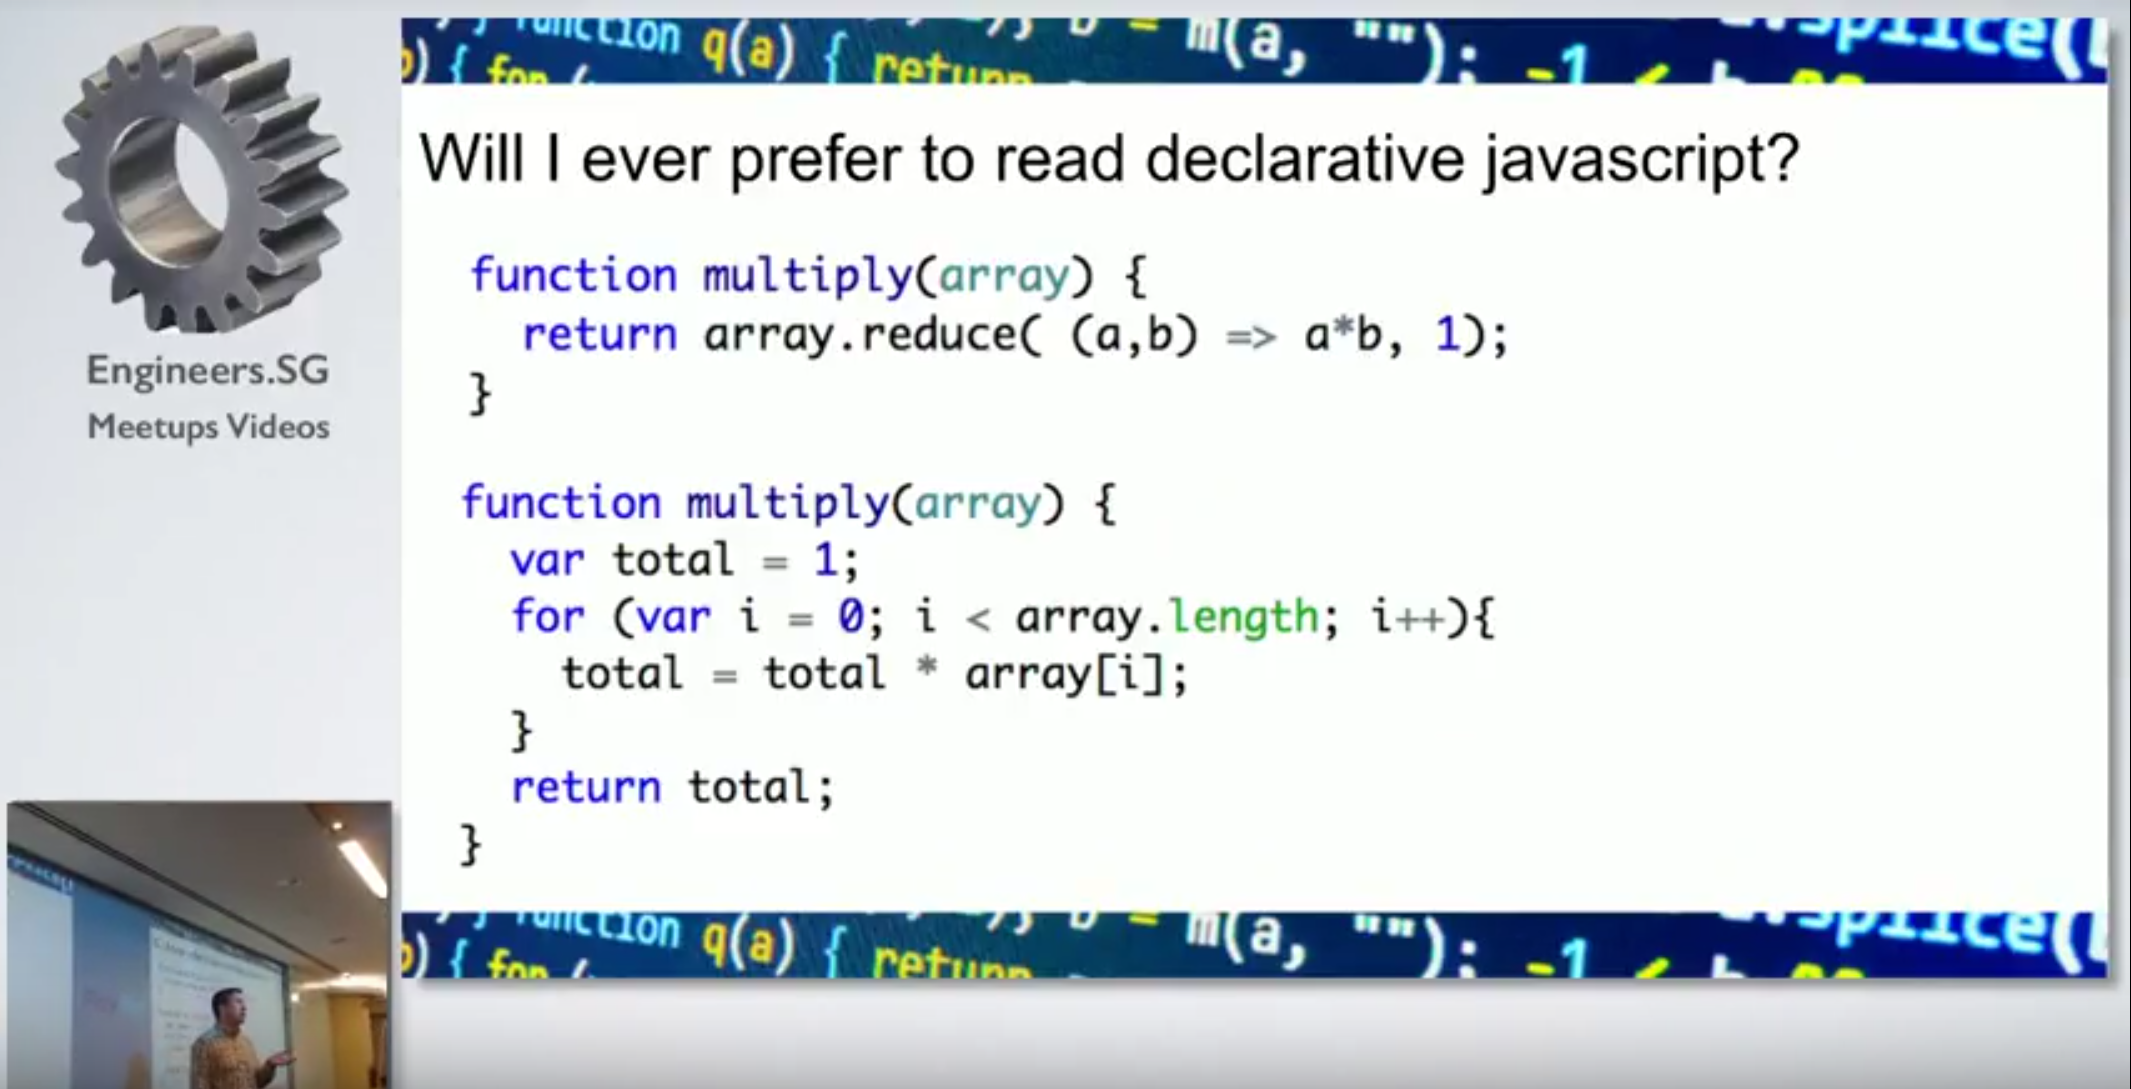
\includegraphics[height=6cm]{fd.png}
\end{center}
\end{frame}

\begin{frame}[fragile]{Agregarea datelor dintr-o colecție (JS)}{
C. Boesch, Declarative vs Imperative Programming - Talk.JS\\
\url{https://www.youtube.com/watch?v=M2e5sq1rnvc}}

\begin{center}
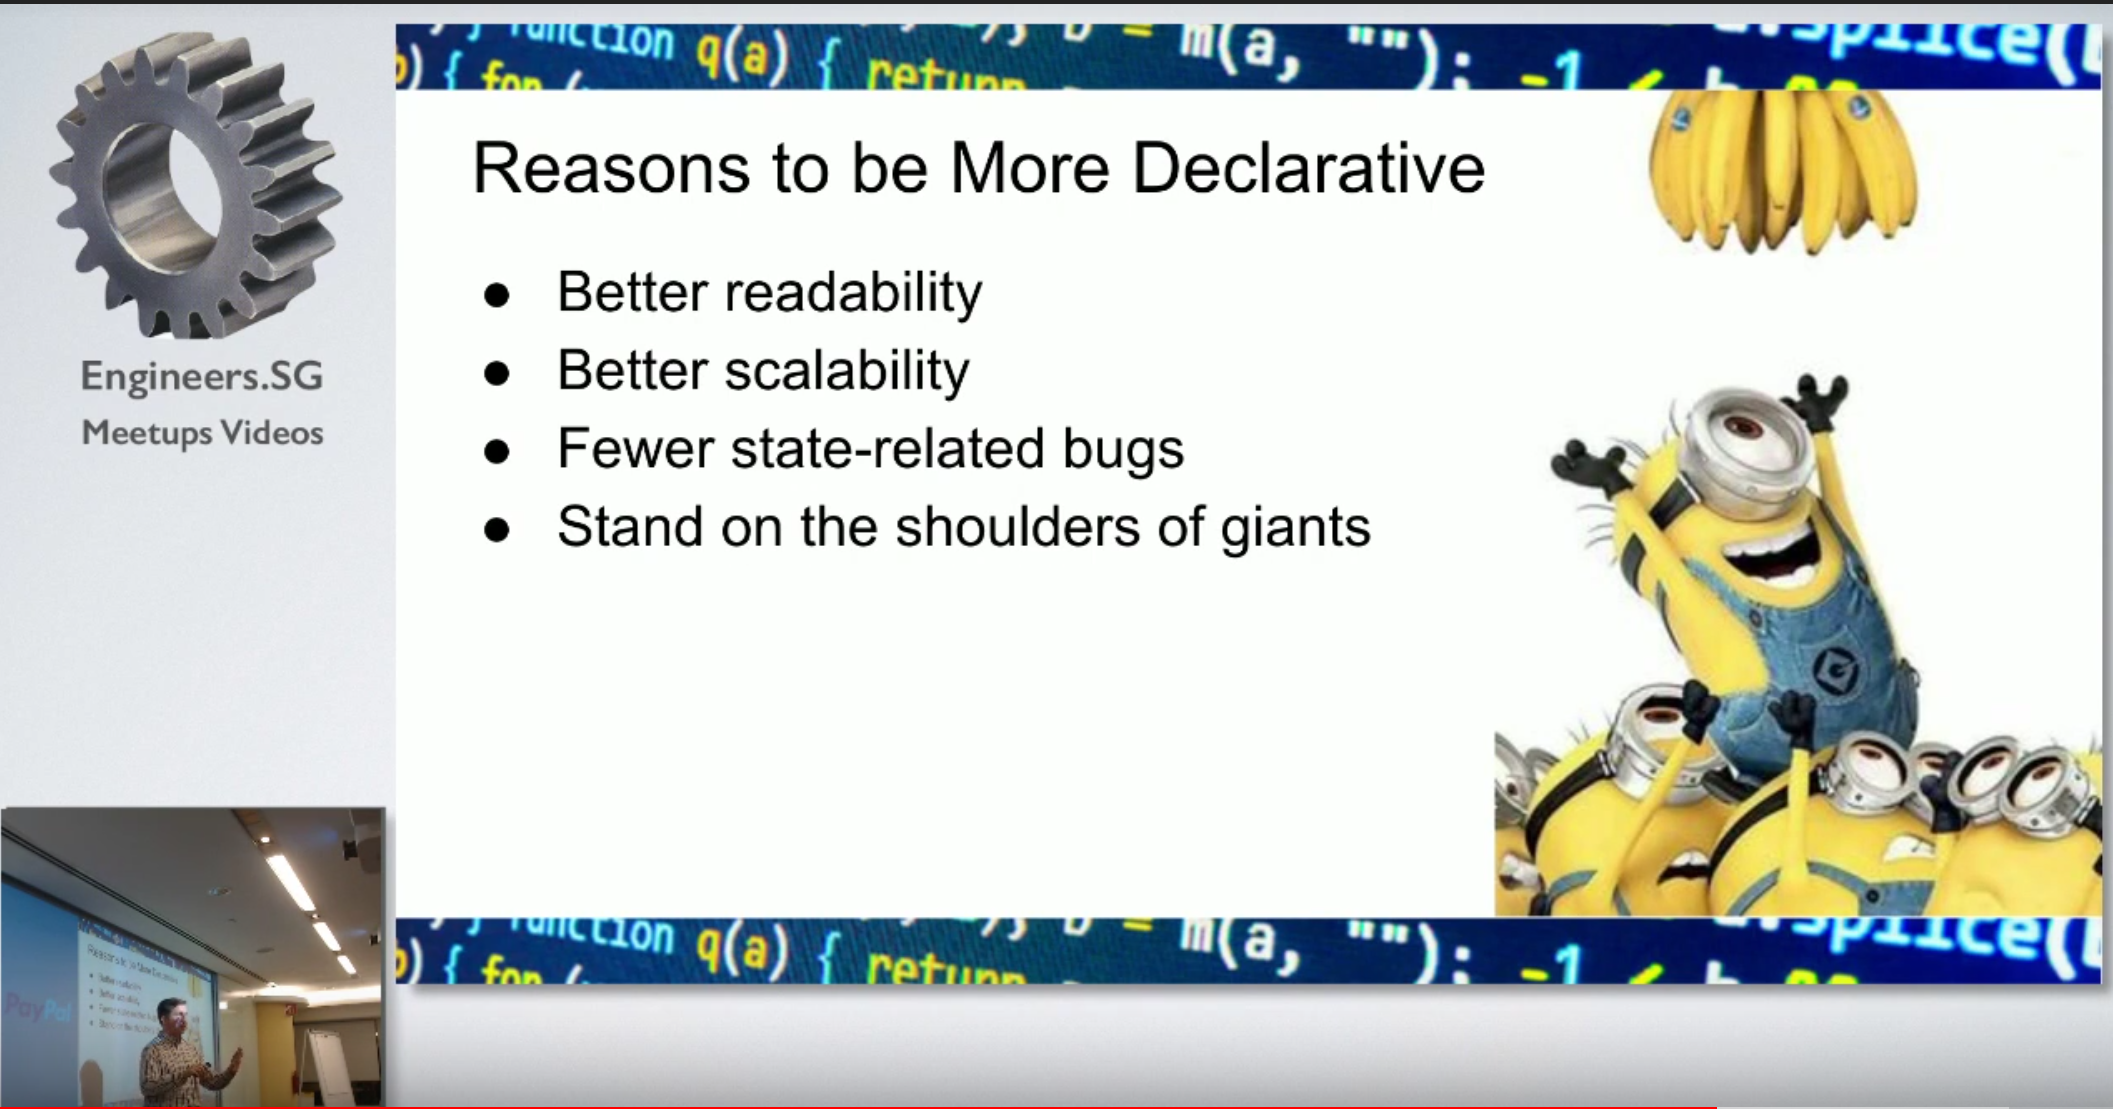
\includegraphics[height=6cm]{giant.png}
\end{center}
\end{frame}



\begin{frame}{Programare funcțională}
\begin{itemize}

\item Programare funcțională în limbajul vostru preferat de programare:
\begin{itemize}
\item Funcții anonime ($\lambda$-abstracții)
  \begin{itemize}
    \item[Java 8] \lstinline[language=java]$(x, y) -> x * y$
    \item[C++ 11] \lstinline[language=c++]$[](x, y) \{return x * y; \}$
    \item[Python] \lstinline[language=python]$lambda x, y: x * y$
    \item[JavaScript] \lstinline[language=javascript]$(x, y) => x * y$
    \vitem[Haskell] \lstinline[language=haskell]$\\x y -> x * y$
  \end{itemize}
\vitem Funcții de procesare a fluxurilor de date: map, filter, reduce/fold
\end{itemize}
\end{itemize}

%\begin{block}{Funcții anonime în Haskell}
% În Haskell, \structure{\textbackslash} e folosit în locul simbolului \structure{$\lambda$} și
% \structure{\lstinline{->}} în locul punctului.
%
%\begin{tabular}{c@{ este  }c}
%$\lambda x. x * x$ & \texttt{\textbackslash x -> x * x}
%\\
%$\lambda x. x > 0$ & \texttt{\textbackslash x -> x > 0}
%\end{tabular}
%\end{block}
%
\end{frame}

\begin{frame}{$\lambda$-calcul}

\begin{itemize}
\item În 1929-1932 Church a propus 
$\lambda$-calculul ca sistem formal pentru logica matematică.
În 1935 a argumentat că orice funcție calculabilă peste numere naturale poate
fi calculată in $\lambda$-calcul.
\[
 \begin{array}{lll}
t= &  x &  \mbox{(variabilă)} \\
 & \mid \lambda x.\, t & \mbox{(abstractizare)}\\
  & \mid t\,\, t & \mbox{(aplicare)}
\end{array}
\]
\item În 1935, independent de Church, Turing a dezvoltat mecanismul de calcul
numit astăzi Mașina Turing. 
În 1936 și el a argumentat câ orice funcție calculabilă peste numere naturale poate
fi calculată de o mașină Turing.
De asemenea, a arătat echivalența celor două modele de calcul.
Această echivalență a constituit o indicație puternică asupra "universalității" 
celor două modele, conducând la ceea ce numim astăzi "Teza Church-Turing".
\end{itemize}
\end{frame}

\begin{frame}[fragile]{Programare funcțională în Haskell}


\begin{block}{De ce Haskell? (din cartea Real World Haskell)
{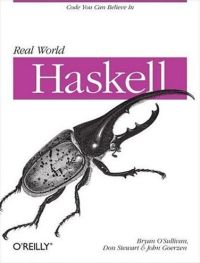
\includegraphics[height=1cm]{rwh.jpg}}}
{The illustration on our cover is of a \href{https://en.wikipedia.org/wiki/Hercules_beetle}{Hercules beetle}. These beetles are among the largest in the world. They are also, in proportion to their size, the strongest animals on Earth, able to lift up to 850 times their own weight. Needless to say, we like the association with a creature that has such a high power-to-weight ratio.}
%\only<3>{ [It] is a deep language and [...] learning it is a hugely rewarding experience.}
\end{block}

\pause
\begin{lstlisting}
primes = sieve [2..]

sieve (p:ps) = p : sieve [ x | x <- ps, x `mod` p /= 0 ]
\end{lstlisting}

%\only<3>{
%\begin{description}
%\item[Nou] Radical diferit de limbajele cu care suntem obișnuiți
%\vitem[Puternic] Cod concis, rapid și sigur
%\vitem[Plăcut] Tehnici elegante pentru rezolvarea de probleme concrete
%\end{description}}
\end{frame}


%\begin{frame}[fragile]{  Exemplu}
%\begin{lstlisting}
%
%
%primes = sieve [2..]
%
%sieve (p:ps) = p : sieve [ x | x <- ps, mod x p /= 0 ]
%\end{lstlisting}
%%\url{https://rosettacode.org/wiki/N-queens_problem}
%%import Control.Monad (foldM)
%%import Data.List ((\\))
%%
%%queens :: Int -> [[Int]]
%%queens n = foldM f [] [1..n]
%%  where
%%     f qs _ = [q:qs | q <- [1..n] \\ qs, q `notDiag` qs]
%%     q `notDiag` qs = and [abs (q - qi) /= i | 
%%                               (qi,i) <- qs `zip` [1..]]
%%% exemplu 
%%% foldM (\x y -> [x+y]) 3 [1,2,3]
%\end{frame}

\begin{frame}{Haskell este un limbaj funcțional pur}
\begin{center}

\includegraphics[height=1cm]{lambda.png} 
\end{center}

\begin{itemize}
\item Funcțiile sunt valori.
\item În loc să modificăm datele existente, calculăm valori noi din valorile existente, folosind funcții
\item Funcțiile sunt \structure{pure}: aceleași rezultate pentru aceleași intrări.
\item O bucată de cod nu poate corupe datele altei bucăți de cod.
\item Distincție clară între părțile pure și cele care comunică cu mediul extern.
\end{itemize}

\begin{itemize}
\item Haskell e folosit în proiecte de Facebook, Google, Microsoft, \ldots
\begin{itemize}
\item Programarea funcțională e din ce în ce mai importantă în industrie 
\item mai multe la \url{https://wiki.haskell.org/Haskell_in_industry}
\end{itemize} 
\item  Oferă suport pentru paralelism și concurență.


\end{itemize}
\end{frame}

\begin{frame}{Haskell este un limbaj elegant}
\begin{itemize}
\item Idei abstracte din matematică devin instrumente puternice practice 
\begin{itemize}
\item recursivitate, compunerea de funcții, functori, monade 
\item folosirea lor permite scrierea de cod compact, modular și reutilizabil
\end{itemize}
\vitem Rigurozitate:  ne forțează să gândim mai mult înainte, dar ne ajută să scriem cod mai corect și mai curat
\vitem Curbă de învățare în trepte
\begin{itemize}
\item Putem scrie programe mici destul de repede
\item Expertiza în Haskell necesită multă \structure{gândire} și \structure{practică}
\item Descoperirea unei lumi noi poate fi un drum distractiv și provocator

\url{http://wiki.haskell.org/Humor}
\end{itemize}
\end{itemize}
\end{frame}



\begin{frame}[fragile]{
\includegraphics[height=0.5cm]{lambda.png} }
\begin{itemize}
\item Haskell e \structure{leneș}: orice calcul e amânat cât de mult posibil
\begin{itemize}
\vitem Schimbă modul de concepere al programelor
\vitem Permite lucrul cu colecții potențial infinite de date precum [1..]
\vitem Evaluarea leneșă poate fi exploatată pentru a reduce timpul de calcul fără a denatura codul
\begin{lstlisting}
firstPrimes k  = take k primes
\end{lstlisting}
\end{itemize}

\item Haskell e \structure{minimalist}: mai puțin cod, în mai puțin timp, și cu mai puține defecte
\begin{itemize}
\vitem
\dots rezolvând totuși problema :-)
\small{
\begin{lstlisting}
numbers = [1,2,3,4,5]
total = foldr (+) 0 numbers
doubled = map (* 2) numbers
\end{lstlisting}}
\end{itemize}
\end{itemize}
\end{frame}




\begin{frame}[fragile]{  Exemplu}
\begin{lstlisting}
qsort :: Ord a => [a] -> [a]

qsort []     = []

qsort (p:xs) = (qsort lesser) ++ [p] ++ (qsort greater)
  where
    (lesser, greater)  = partition (< p) xs
\end{lstlisting}

\end{frame}

\end{section}

\begin{frame}
  \vfill
  \centering



  \begin{beamercolorbox}[sep=8pt,center,shadow=true,rounded=true]{title}
    \usebeamerfont{title} Succes! \par%
  \end{beamercolorbox}
  \vfill
  \end{frame}
\end{document}






